% ============================================================
% Project Work 2 -- BSc Applied Digital Life Sciences, ZHAW LSFM
% Structure according to "Arbeitsanleitung fuer die Abfassung von
% studentischen Arbeiten im Bereich Life Sciences" (N-AA)
% ============================================================
\documentclass[11pt,a4paper,oneside]{report}

% ------------------------------------------------------------
% Metadata (used on title page, imprint and header)
% ------------------------------------------------------------
\newcommand{\thesistitle}{Navigation and Environmental Mapping for an Autonomous Mobile Robot}
\newcommand{\thesissubtitle}{}
\newcommand{\thesistype}{Project Work 2}
\newcommand{\authorfirst}{Tim}
\newcommand{\authorlast}{Badertscher}
\newcommand{\degreeprogramme}{Bachelor's Degree Programme Applied Digital Life Sciences}
\newcommand{\specialisation}{Specialisation Digital Labs and Production}
\newcommand{\minors}{Minors Ecology, Geodata Processing and Image Processing}
\newcommand{\submissiondate}{10 December 2026}
\newcommand{\institute}{Institute of Computational Life Sciences}

% ------------------------------------------------------------
% Packages
% ------------------------------------------------------------
\usepackage[T1]{fontenc}
\usepackage[utf8]{inputenc}
\usepackage[english]{babel}
\usepackage[a4paper,margin=2.5cm,headheight=14pt]{geometry}

% Sans-serif font similar to Arial (guideline: e.g. Arial 11 pt)
\usepackage[scaled=0.92]{helvet}
\renewcommand{\familydefault}{\sfdefault}
\usepackage[italic]{mathastext}

% Line spacing (guideline: max. 1.5)
\usepackage{setspace}
\setstretch{1.2}

\usepackage{graphicx}
\usepackage{subcaption}
\usepackage{booktabs}
\usepackage{tabularx}
\usepackage{float}
\usepackage[font=small,labelfont=bf]{caption}
\usepackage{siunitx}
\usepackage{amsmath}
\usepackage{xcolor}
\usepackage{listings}
\usepackage{tikz}
\usetikzlibrary{arrows.meta,positioning,fit,backgrounds,calc}
\usepackage{fancyhdr}
\usepackage{titlesec}
\usepackage[nottoc,notlot,notlof,numbib]{tocbibind}
\usepackage[numbers,square,sort&compress]{natbib}
\usepackage[hidelinks]{hyperref}
\urlstyle{same}

% ------------------------------------------------------------
% Layout
% ------------------------------------------------------------
% Compact chapter headings
\titleformat{\chapter}[hang]{\normalfont\LARGE\bfseries}{\thechapter}{0.8em}{}
\titlespacing*{\chapter}{0pt}{0pt}{1.2em}

% Header: ZHAW LSFM, type of work, author; footer: page number
\pagestyle{fancy}
\fancyhf{}
\fancyhead[L]{\small ZHAW LSFM -- \thesistype}
\fancyhead[R]{\small \authorfirst\ \authorlast}
\fancyfoot[C]{\small\thepage}
\renewcommand{\headrulewidth}{0.4pt}
\fancypagestyle{plain}{\fancyhf{}\fancyhead[L]{\small ZHAW LSFM -- \thesistype}\fancyhead[R]{\small \authorfirst\ \authorlast}\fancyfoot[C]{\small\thepage}}

% Labels according to the guideline ("Fig." / "Tab.")
\addto\captionsenglish{
  \renewcommand{\figurename}{Fig.}
  \renewcommand{\tablename}{Tab.}
  \renewcommand{\bibname}{References}
}

% Avoid lines sticking out into the margin (long \texttt words)
\setlength{\emergencystretch}{3em}

% ------------------------------------------------------------
% Helpers
% ------------------------------------------------------------
% Open points that still have to be filled in or checked
\newcommand{\todo}[1]{\textcolor{red}{\textbf{[TODO: #1]}}}

\sisetup{per-mode=symbol}

\definecolor{codebg}{RGB}{248,248,248}
\definecolor{codecomment}{RGB}{90,120,90}
\definecolor{codekeyword}{RGB}{30,60,150}
\lstset{
  basicstyle=\ttfamily\footnotesize,
  backgroundcolor=\color{codebg},
  commentstyle=\color{codecomment},
  keywordstyle=\color{codekeyword}\bfseries,
  stringstyle=\color{black!70},
  frame=single,
  rulecolor=\color{black!20},
  breaklines=true,
  columns=fullflexible,
  keepspaces=true,
  showstringspaces=false,
  numbers=left,
  numberstyle=\tiny\color{black!50},
  captionpos=t
}
\renewcommand{\lstlistingname}{Listing}
\lstdefinelanguage{json}{morestring=[b]"}

% ============================================================
\begin{document}

% ---------------- Preliminaries (not numbered) --------------
\pagenumbering{roman}
% Title page according to the template in Annex 2 of the guideline
\begin{titlepage}
  \thispagestyle{empty}
  \centering
  \setstretch{1.15}

  {\large\bfseries ZURICH UNIVERSITY OF APPLIED SCIENCES\\
  SCHOOL OF LIFE SCIENCES AND FACILITY MANAGEMENT\\
  \MakeUppercase{\institute}\par}

  \vspace{3.5cm}

  {\LARGE\bfseries \thesistitle\par}

  \vspace{2.5cm}

  {\Large \thesistype\par}

  \vspace{2cm}

  {\large by\par}
  \vspace{0.3cm}
  {\large\bfseries \authorlast, \authorfirst\par}
  \vspace{0.3cm}
  {\large \degreeprogramme\\
  Submission date: \submissiondate\\
  \specialisation\\
  \minors\par}

  \vfill

  \raggedright
  {\large\bfseries Supervisor:\par}
  \vspace{0.2cm}
  {\large \todo{academic title} Christian Glahn\\
  ZHAW Zurich University of Applied Sciences, \institute\\
  \todo{address, place}\par}
\end{titlepage}

% Imprint on the back of the title page: keywords, citation suggestion, institute
\thispagestyle{empty}
\vspace*{\fill}
\noindent
\begin{tabularx}{\textwidth}{@{}l X@{}}
  \textbf{Keywords} & Autonomous mobile robot, ROS2, odometry, inertial measurement unit, lidar, SLAM, navigation, collision avoidance, Agriculture~4.0 \\[0.8em]
  \textbf{Citation suggestion} & \authorlast, \authorfirst\ (2026). \emph{\thesistitle} [\thesistype, unpublished]. Zurich University of Applied Sciences, ZHAW. \\[0.8em]
  \textbf{Institute} & Zurich University of Applied Sciences (ZHAW), School of Life Sciences and Facility Management, \institute \\
\end{tabularx}
\clearpage

% Abstract (English) and Zusammenfassung (German) -- not numbered.
% Guideline: 0.5 to max. 1 A4 page each, no citations; field, objective,
% methods, results and conclusions. Write at the end of the project.

\chapter*{Abstract}
\thispagestyle{fancy}

\todo{Write at the end of the project (0.5--1 page, no citations). Cover: field and problem, research question and objectives, methods, main results with numbers, conclusions.}

\chapter*{Zusammenfassung}
\thispagestyle{fancy}

\todo{Abstract auf Deutsch}


\tableofcontents
% List of abbreviations -- not numbered, alphabetical
\chapter*{List of Abbreviations}
\thispagestyle{fancy}

\begin{tabularx}{\textwidth}{@{}l X@{}}
  ESP32   & Microcontroller (Espressif) used as sub-controller of the robot \\
  IMU     & Inertial measurement unit \\
  JSON    & JavaScript Object Notation \\
  LTS     & Long-term support \\
  MPPI    & Model predictive path integral (controller of Nav2) \\
  Nav2    & ROS2 navigation stack \\
  PID     & Proportional--integral--derivative (controller) \\
  REP     & ROS Enhancement Proposal \\
  ROS2    & Robot Operating System 2 \\
  SLAM    & Simultaneous localisation and mapping \\
  TF      & Transform (coordinate frame system of ROS2) \\
  UART    & Universal asynchronous receiver-transmitter (serial interface) \\
  URDF    & Unified Robot Description Format \\
\end{tabularx}


% ---------------- Main part ---------------------------------
\cleardoublepage
\pagenumbering{arabic}
\chapter{Introduction}
\label{ch:introduction}

\section{Background}

Robotics is seen as an important technology for the future of agriculture, for example to address the shortage of workers and to reduce environmental impacts such as soil compaction and the use of pesticides~\citep{duckett2018}. Typical applications of agricultural robots are weeding, harvesting and the monitoring of crops~\citep{oliveira2021}. Autonomous mobile robots can take over such repetitive tasks. Before a robot can do any of these tasks, it has to know its surroundings and be able to move in them safely without hitting obstacles. This project therefore focuses on these basic capabilities, mapping and navigation, on which later tasks can build.

This project builds on a previous project at the EDXI Lab of ZHAW, which looked at an autonomous robot for plant management on green rooftops with photovoltaic installations~\citep{graham2024}. In that project, a robot chassis, a basic control logic and design specifications were developed, and a digital twin of the robot was built with ROS2. The real robot did not drive autonomously yet: it had no sensors for the environment and no wheel encoders, so odometry, mapping and navigation were not possible. The previous work also recommended using a long-term support release of ROS2 instead of the unstable Rolling distribution.

For this project, the EDXI Lab provided a commercial robot platform, a Waveshare RaspRover, which already includes wheel encoders, an IMU and a motor controller, together with an RPLIDAR A2M12 lidar sensor.

\section{Objectives}

The objective of this project is to implement robot control for movement and environmental mapping, so that the robot can map and navigate the Schlosshof of ZHAW Wädenswil using ROS2, with all processing done on the robot itself (edge computing). Two results are expected:

\begin{enumerate}
  \item \textbf{Robot and sensor control}
  \item \textbf{Collision avoidance and mapping} with the lidar sensor
\end{enumerate}

The work follows the guiding questions from the project outline (Tab.~\ref{tab:questions}).

\begin{table}[H]
  \centering
  \small
  \caption{Guiding questions of the project and the chapters in which they are answered.}
  \label{tab:questions}
  \begin{tabularx}{\textwidth}{@{}l X l@{}}
    \toprule
    \textbf{Phase} & \textbf{Guiding question} & \textbf{Chapter} \\
    \midrule
    Preparation        & What approaches exist for mapping and navigation of mobile robots? & \ref{ch:theory} \\
                       & What are the challenges of self-driving robots? & \ref{ch:theory} \\
    \midrule
    Setup of robot     & How does the robot move? & \ref{ch:methods}, \ref{ch:results} \\
    and sensors        & Which sensors and actuators does the robot have? & \ref{ch:methods} \\
                       & How do the robot's components communicate with each other? & \ref{ch:methods} \\
    \midrule
    Mapping and        & How can the robot capture and map its environment? & \ref{ch:methods}, \ref{ch:results} \\
    navigation         & How does the robot determine its position on the map? & \ref{ch:methods}, \ref{ch:results} \\
                       & How does the robot detect and avoid obstacles? & \ref{ch:methods}, \ref{ch:results} \\
                       & How can the robot reach a given position? & \ref{ch:methods}, \ref{ch:results} \\
    \midrule
    Evaluation         & How accurate is the generated map? & \ref{ch:results}, \ref{ch:discussion} \\
                       & How reliably does the robot reach its target? & \ref{ch:results}, \ref{ch:discussion} \\
                       & What are the limitations of the system? & \ref{ch:discussion} \\
    \bottomrule
  \end{tabularx}
\end{table}

\section{Scope}

The project only covers the perception of the environment and the movement of the robot. Plant detection, additional actuators and the robotic arm that is developed for the robot by students in Madrid are not part of this work.
\chapter{Theoretical Background}
\label{ch:theory}

\section{ROS2 basics}

ROS2 is a framework for robot software. A program in ROS2 is split into \emph{nodes}, and each node has one task, for example reading a sensor or controlling the motors. Nodes exchange messages over named channels called \emph{topics}. A node can publish messages on a topic, and any other node can subscribe to it~\citep{ros2_jazzy}. Each topic has a fixed message type, for example \texttt{sensor\_msgs/LaserScan} for a lidar scan or \texttt{geometry\_msgs/Twist} for a velocity command. Settings of a node are given as \emph{parameters}, and several nodes can be started together with a \emph{launch file}~\citep{ros2_jazzy}.

The positions of the robot and its sensors are described with coordinate frames. The library \texttt{tf2} keeps track of the transforms between these frames, so that for example a lidar point can be converted from the lidar frame into the map frame~\citep{ros2_jazzy}. REP~103 defines SI units and a coordinate system with $x$ forward, $y$ to the left and $z$ up~\citep{rep103}. REP~105 defines the standard frames of a mobile robot~\citep{rep105}:
\begin{itemize}
  \item \texttt{base\_link} is fixed to the robot,
  \item \texttt{odom} is a frame in which the robot position changes smoothly but drifts over time (odometry),
  \item \texttt{map} is a frame in which the robot position is corrected, for example by SLAM.
\end{itemize}
The transform chain is therefore \texttt{map}~$\rightarrow$~\texttt{odom}~$\rightarrow$~\texttt{base\_link}~$\rightarrow$~sensor frames.

\section{Mapping and navigation}
\label{sec:theory_slam}

\paragraph{SLAM Toolbox.} SLAM (simultaneous localisation and mapping) means that the robot builds a map and at the same time estimates its own position in this map. In this work, the SLAM Toolbox was used, a ROS2 package for 2D SLAM with a lidar~\citep{slam_toolbox}. It matches each new laser scan with the previous scans (scan matching), stores the robot poses in a pose graph and corrects the graph when the robot comes back to a place it has already seen (loop closure). The odometry of the robot is used as the starting point for the scan matching. SLAM Toolbox publishes the map on \texttt{/map} and the transform \texttt{map}~$\rightarrow$~\texttt{odom}. It can run in a synchronous mode, where every scan is processed, or in an asynchronous mode, where a new scan is only processed when the previous one is finished~\citep{slam_toolbox}.

\paragraph{Nav2.} Nav2 is the navigation stack of ROS2~\citep{nav2_docs}. It consists of several nodes:
\begin{itemize}
  \item the \emph{planner server} plans a path from the robot to the goal on a global cost map,
  \item the \emph{controller server} follows this path and calculates velocity commands using a local cost map around the robot,
  \item the \emph{behavior tree navigator} receives the goal and coordinates the other nodes,
  \item the \emph{behavior server} runs recovery behaviours, for example turning on the spot or backing up, when the robot is stuck,
  \item the \emph{velocity smoother} limits the velocities and accelerations before the command is sent to the robot on \texttt{/cmd\_vel}.
\end{itemize}
The cost maps contain the obstacles from the map and from the current laser scan, with a safety zone around them (inflation), so that the planned path keeps a distance to obstacles~\citep{nav2_docs}. One of the available controllers is the MPPI controller (model predictive path integral). It samples many possible trajectories, rates them with several criteria (e.g.\ distance to the path and to obstacles) and chooses the best one~\citep{nav2_docs}.

Nav2 can also be used while the map is still being created. In this case, SLAM Toolbox provides the map and the transform \texttt{map}~$\rightarrow$~\texttt{odom}, and no separate localisation is needed~\citep{nav2_slam}.

\paragraph{Visualisation.} Foxglove is a tool for visualising robot data. The \texttt{foxglove\_bridge} runs as a node on the robot and provides the ROS2 topics over a WebSocket connection, so that the Foxglove application on another computer can display them and also publish messages~\citep{foxglove_bridge}.

\section{Challenges of self-driving robots}
\label{sec:challenges}

\todo{To be written with literature.}

\chapter{Materials and Methods}
\label{ch:methods}

\section{Robot platform}
\label{sec:platform}

A Waveshare RaspRover with a Raspberry Pi~5 was used~\citep{waveshare_rasprover}. Instead of rebuilding the chassis from the previous work~\citep{graham2024}, this platform was chosen because it already has four driven wheels with encoders, an inertial measurement unit (IMU), a voltage measurement and its own motor controller. A Slamtec RPLIDAR A2M12 lidar was used to sense the environment~\citep{slamtec_a2m12}.

The robot has two controllers (Fig.~\ref{fig:architecture}). The Raspberry Pi~5 is the main computer and runs ROS2 and all other software. An ESP32 microcontroller on the Waveshare driver board controls the motors and reads the sensors on the board~\citep{waveshare_driver}. The Raspberry Pi is plugged onto the driver board with its 40-pin header, which provides both the \SI{5}{\volt} supply and the UART connection to the ESP32. Table~\ref{tab:components} lists the sensors and actuators.

\begin{figure}[H]
  \centering
  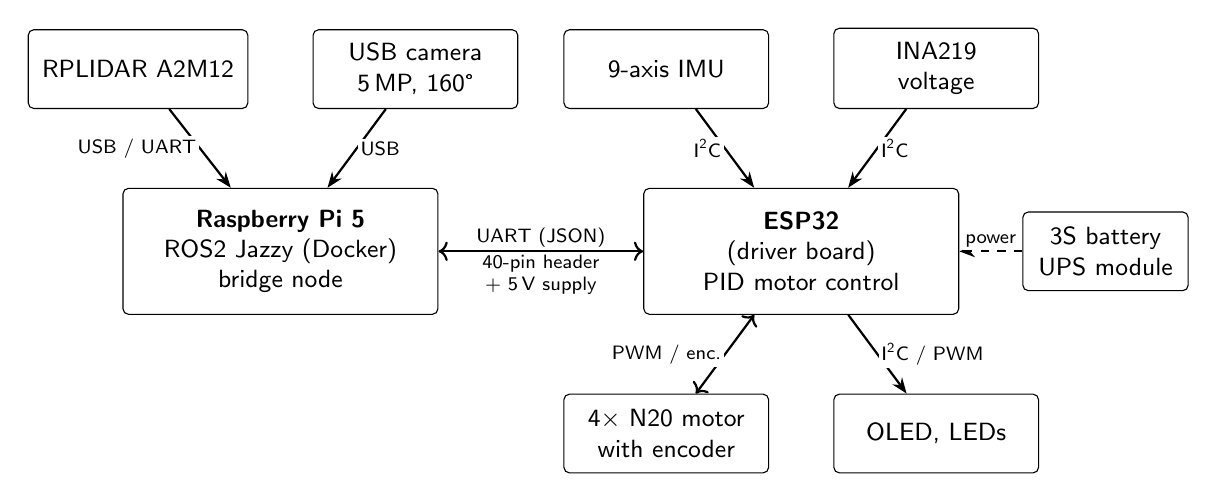
\begin{tikzpicture}[
      font=\small,
      box/.style={draw, rounded corners=2pt, align=center, minimum height=1cm, inner sep=5pt, fill=white},
      comp/.style={box, minimum width=2.6cm},
      arr/.style={-{Stealth[length=2mm]}, thick},
      lbl/.style={font=\scriptsize, fill=white, inner sep=1pt}
    ]
    \node[comp, minimum width=4.0cm, minimum height=1.6cm] (pi) {\textbf{Raspberry Pi 5}\\ROS2 Jazzy (Docker)\\bridge node};
    \node[comp, minimum width=4.0cm, minimum height=1.6cm, right=2.6cm of pi] (esp) {\textbf{ESP32}\\(driver board)\\PID motor control};
    \node[comp, above left=1.0cm and -1.6cm of pi] (lidar) {RPLIDAR A2M12};
    \node[comp, above right=1.0cm and -1.6cm of pi] (cam) {USB camera\\5\,MP, 160°};
    \node[comp, above left=1.0cm and -1.6cm of esp] (imu) {9-axis IMU};
    \node[comp, above right=1.0cm and -1.6cm of esp] (ina) {INA219\\voltage};
    \node[comp, below left=1.0cm and -1.6cm of esp] (mot) {4$\times$ N20 motor\\with encoder};
    \node[comp, below right=1.0cm and -1.6cm of esp] (oled) {OLED, LEDs};
    \node[comp, minimum width=2.1cm, right=0.8cm of esp] (bat) {3S battery\\UPS module};
    \draw[arr, <->] (pi) -- node[lbl, above] {UART (JSON)} node[lbl, below, align=center] {40-pin header\\+ \SI{5}{\volt} supply} (esp);
    \draw[arr] (lidar) -- node[lbl, left] {USB / UART} (pi);
    \draw[arr] (cam) -- node[lbl, right] {USB} (pi);
    \draw[arr] (imu) -- node[lbl, left] {I\textsuperscript{2}C} (esp);
    \draw[arr] (ina) -- node[lbl, right] {I\textsuperscript{2}C} (esp);
    \draw[arr, <->] (esp) -- node[lbl, left] {PWM / enc.} (mot);
    \draw[arr] (esp) -- node[lbl, right] {I\textsuperscript{2}C / PWM} (oled);
    \draw[arr, dashed] (bat) -- node[lbl, above] {power} (esp);
  \end{tikzpicture}
  \caption{Hardware architecture of the robot.}
  \label{fig:architecture}
\end{figure}


\begin{table}[H]
  \centering
  \small
  \caption{Sensors and actuators of the robot.}
  \label{tab:components}
  \begin{tabularx}{\textwidth}{@{}l l l X@{}}
    \toprule
    \textbf{Type} & \textbf{Component} & \textbf{Interface} & \textbf{Data / function} \\
    \midrule
    Sensor   & RPLIDAR A2M12             & UART over USB   & 360° 2D scan~\citep{slamtec_a2m12} \\
    Sensor   & Wheel encoders            & ESP32           & Speed and distance of each side \\
    Sensor   & 9-axis IMU                & I\textsuperscript{2}C, ESP32 & Acceleration, angular rate and magnetic field~\citep{waveshare_driver} \\
    Sensor   & INA219                    & I\textsuperscript{2}C, ESP32 & Battery voltage~\citep{waveshare_driver} \\
    Sensor   & USB camera                & USB             & Not used in this work \\
    Actuator & 4 DC gear motors          & ESP32           & Drive (skid steering) \\
    Actuator & Lidar motor               & Lidar           & Rotation of the lidar head \\
    \bottomrule
  \end{tabularx}
\end{table}

The robot is powered by three 18650 lithium-ion cells (3S) with a UPS module, so it can be charged while it is running~\citep{waveshare_rasprover}.

\section{Software environment}
\label{sec:software}

The Raspberry Pi runs the Raspberry Pi OS image from Waveshare (Debian Bookworm, 64-bit), which includes a web application for remote control. This web application blocks the serial port to the ESP32, so its autostart entry in \texttt{crontab} was disabled.

ROS2 Jazzy Jalisco was chosen because it is a long-term support (LTS) release~\citep{ros2_jazzy}. This also follows the recommendation of the previous work to use an LTS release instead of Rolling~\citep{graham2024}. ROS2 Jazzy is made for Ubuntu~24.04 and not for Raspberry Pi OS. Therefore, ROS2 was run in a Docker container based on the official image \texttt{ros:jazzy-ros-base}. This way, the manufacturer image stays unchanged. The container was started with host networking (for the visualisation on the laptop), with access to the device files (serial port of the ESP32 and the lidar) and with the ROS2 workspace mounted from the Raspberry Pi, so the code is not lost when the container is deleted (Appendix~\ref{app:code}).

\section{Communication with the ESP32}
\label{sec:protocol}

The Raspberry Pi communicates with the ESP32 over UART (\texttt{/dev/ttyAMA0}, \SI{115200}{baud}). Each message is one line of JSON, and the key \texttt{T} gives the command type~\citep{waveshare_json}. The following commands were used (overview in Appendix~\ref{app:commands}):

\begin{itemize}
  \item \texttt{\{"T":900,"main":1,"module":0\}} sets the chassis type to RaspRover. This has to be sent after every start, otherwise the direction and speed of the wheels are wrong.
  \item \texttt{\{"T":13,"X":$v$,"Z":$\omega$\}} sets the linear velocity $v$ in \si{\metre\per\second} and the angular velocity $\omega$ in \si{\radian\per\second}.
  \item \texttt{\{"T":131,"cmd":1\}} switches on the continuous feedback.
\end{itemize}

The firmware has a heartbeat function, which stops the motors when no new drive command arrives for some time~\citep{waveshare_json}. With continuous feedback switched on, the ESP32 sends a feedback message (\texttt{"T":1001}) with wheel speeds, distance counters, raw IMU values and the battery voltage (example in Appendix~\ref{app:rawdata}). The units of these values are not documented, so they had to be determined with tests (Section~\ref{sec:calibration_method}).

\section{ROS2 bridge node}
\label{sec:bridge}

Waveshare does not provide a ROS2 driver for the robot. Therefore, a bridge node (\texttt{rasprover\_bridge}) was written in Python (Fig.~\ref{fig:bridge}, code in Appendix~\ref{app:code}). It translates between the standard ROS2 topics and the JSON commands of the ESP32, so that standard packages like SLAM Toolbox and Nav2 can use the robot.

\begin{figure}[H]
  \centering
  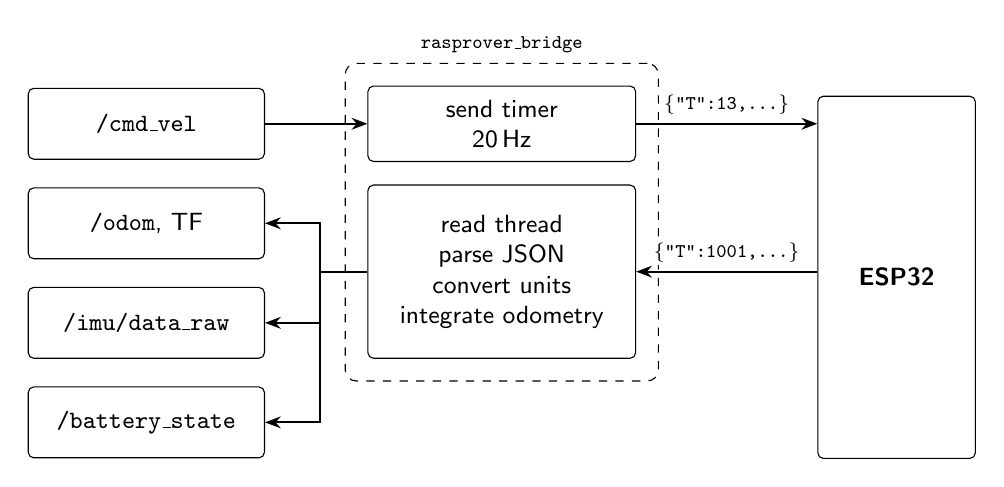
\begin{tikzpicture}[
      font=\small,
      box/.style={draw, rounded corners=2pt, align=center, minimum height=0.9cm, inner sep=5pt, fill=white},
      arr/.style={-{Stealth[length=2mm]}, thick},
      lbl/.style={font=\scriptsize, fill=white, inner sep=1pt}
    ]
    \node[box, minimum width=3.0cm] (cmd) {\texttt{/cmd\_vel}};
    \node[box, minimum width=3.0cm, below=0.35cm of cmd] (odom) {\texttt{/odom}, TF};
    \node[box, minimum width=3.0cm, below=0.35cm of odom] (imu) {\texttt{/imu/data\_raw}};
    \node[box, minimum width=3.0cm, below=0.35cm of imu] (bat) {\texttt{/battery\_state}};
    \node[box, right=1.3cm of cmd, minimum width=3.4cm] (timer) {send timer\\\SI{20}{\hertz}};
    \node[box, right=1.3cm of imu, minimum width=3.4cm, yshift=0.65cm, minimum height=2.2cm] (reader) {read thread\\parse JSON\\convert units\\integrate odometry};
    \node[box, right=2.3cm of timer, minimum width=2.0cm, minimum height=4.6cm, yshift=-1.95cm] (esp) {\textbf{ESP32}};
    \begin{scope}[on background layer]
      \node[draw, dashed, rounded corners, fit=(timer)(reader), inner sep=8pt, label={[font=\scriptsize]above:\texttt{rasprover\_bridge}}] {};
    \end{scope}
    \draw[arr] (cmd) -- (timer);
    \draw[arr] (timer) -- node[lbl, above=2pt] {\texttt{\{"T":13,...\}}} (timer -| esp.west);
    \draw[arr] (reader -| esp.west) -- node[lbl, above=2pt] {\texttt{\{"T":1001,...\}}} (reader);
    \draw[arr] (reader.west) -- ++(-0.6,0) |- (odom);
    \draw[arr] (reader.west) -- ++(-0.6,0) |- (imu);
    \draw[arr] (reader.west) -- ++(-0.6,0) |- (bat);
  \end{tikzpicture}
  \caption{Structure of the bridge node.}
  \label{fig:bridge}
\end{figure}


\paragraph{Structure.} A timer sends the current drive command to the ESP32 every \SI{50}{\milli\second}. A separate thread continuously reads the serial port and processes every feedback message. A lock makes sure that two commands are not written at the same time.

\paragraph{Start.} At the start, the node sets the chassis type and switches on the feedback. The robot then has to stand still for \SI{2}{\second} while the node averages the gyroscope values to get the offset $b$. During this time, no drive commands are sent.

\paragraph{Commands.} The node takes the linear velocity $v$ and the angular velocity $\omega$ from \texttt{/cmd\_vel} and sends them as a \texttt{T:13} command. The ESP32 converts them to wheel speeds. If no message arrives for \SI{0.5}{\second}, the node sends a stop command. Together with the heartbeat of the ESP32, the robot therefore stops if either the program sending the commands or the bridge node itself crashes.

\paragraph{Odometry.} Each feedback message is converted to SI units (Tab.~\ref{tab:feedback}). Because the robot slips a lot when it turns (Section~\ref{sec:calibration_results}), the distance is taken from the wheel encoders, but the heading is taken from the gyroscope. With the changes of the distance counters $\Delta n_l$ and $\Delta n_r$, the scale factor $s$, the angular rate $\omega_z$ (without offset) and the time step $\Delta t$:

\begin{align}
  d &= \tfrac{1}{2}\,s\,(\Delta n_l + \Delta n_r), \qquad \psi_k = \psi_{k-1} + \omega_z\,\Delta t, \\
  x_k &= x_{k-1} + d\,\cos\!\left(\psi_{k-1} + \tfrac{1}{2}\,\omega_z\,\Delta t\right), \qquad
  y_k = y_{k-1} + d\,\sin\!\left(\psi_{k-1} + \tfrac{1}{2}\,\omega_z\,\Delta t\right).
\end{align}

The distance counters are reset when the ESP32 restarts. Therefore, only the differences are used, and jumps of more than \SI{0.5}{\metre} between two messages are ignored.

\paragraph{Topics.} Table~\ref{tab:topics} shows the topics of the bridge node. The frames follow REP~103 and REP~105~\citep{rep103,rep105}. The conversion factors, the port, the command rate and the timeout are ROS2 parameters, so they can be changed without changing the code.

\begin{table}[H]
  \centering
  \small
  \caption{Topics of the bridge node.}
  \label{tab:topics}
  \begin{tabularx}{\textwidth}{@{}l l X@{}}
    \toprule
    \textbf{Topic} & \textbf{Message type} & \textbf{Content} \\
    \midrule
    \texttt{/cmd\_vel} (input) & \texttt{geometry\_msgs/Twist}       & Drive commands \\
    \texttt{/odom}             & \texttt{nav\_msgs/Odometry}         & Position and velocity from encoders and gyroscope \\
    \texttt{/tf}               & \texttt{odom} $\rightarrow$ \texttt{base\_link} & Position of the robot relative to its start position \\
    \texttt{/imu/data\_raw}    & \texttt{sensor\_msgs/Imu}           & Acceleration and angular rate \\
    \texttt{/battery\_state}   & \texttt{sensor\_msgs/BatteryState}  & Battery voltage and rough charge level \\
    \bottomrule
  \end{tabularx}
\end{table}

\section{Calibration of the sensor values}
\label{sec:calibration_method}

The units and scale factors of the feedback values were determined with simple tests on a smooth floor indoors. Distances were measured with a measuring tape, angles were estimated by eye. Because the ESP32 sends feedback continuously, the serial input buffer was cleared before each reading, so that the newest message was used.

\begin{itemize}
  \item \textbf{Wheel speed and distance:} The robot drove forward and backward with \SI{0.3}{\metre\per\second} for about \SI{3.3}{\second}. The values \texttt{L}/\texttt{R} and the changes of the counters \texttt{odl}/\texttt{odr} were recorded and compared with the measured distance.
  \item \textbf{Accelerometer:} The vertical acceleration was read while the robot was standing on a flat floor and while it was lying upside down.
  \item \textbf{Gyroscope offset:} The mean of 30 values of the vertical angular rate was calculated while the robot was standing still.
  \item \textbf{Gyroscope scale:} The robot turned on the spot for \SI{3}{\second} with a commanded angular velocity of \SI{1.5}{\radian\per\second}. The values (without offset) were integrated over time with the trapezoidal rule and divided by the estimated rotation angle.
\end{itemize}

\section{Test of the bridge node}
\label{sec:validation_method}

The rate of \texttt{/odom} was measured with \texttt{ros2 topic hz}. After that, the robot was driven manually with \texttt{teleop\_twist\_keyboard} (\SI{0.2}{\metre\per\second}, \SI{1.05}{\radian\per\second}) in two tests, and the position on \texttt{/odom} was recorded:

\begin{itemize}
  \item \textbf{Straight drive:} After restarting the node, the robot drove straight ahead for about \SI{1}{\metre}. The odometry was compared with the measured distance and the visible deviation from a straight line.
  \item \textbf{Turn:} The robot turned to the left on the spot by about \SI{90}{\degree}. The heading was calculated from the orientation quaternion as $\psi = 2\arcsin(q_z)$, which is valid for a rotation around the vertical axis only.
\end{itemize}

The drift of the heading while standing still was read from the recordings before and after the movements.

\section{Lidar integration}
\label{sec:lidar_method}

The lidar was connected to a USB port of the Raspberry Pi with the USB--UART adapter that comes with the sensor (\texttt{/dev/ttyUSB0}). The ROS2 driver \texttt{sllidar\_ros2} from Slamtec was built from source in the container and started with its launch file for the A2M12 (\SI{256000}{baud}). The driver publishes the scan on \texttt{/scan} (\texttt{sensor\_msgs/LaserScan}) in the frame \texttt{laser}.

The Raspberry Pi~5 limits the current of its USB ports when it is not powered by the official power supply. Because the Pi is powered by the driver board of the robot, this limit was switched off with the setting \texttt{usb\_max\_current\_enable=1} in \texttt{/boot/firmware/config.txt} (Section~\ref{sec:lidar_results}). Undervoltage was checked with \texttt{vcgencmd get\_throttled}.

The scan was checked with \texttt{ros2 topic hz} and by holding a hand at a known position in front of the lidar. For the visualisation, Foxglove was used, a tool for visualising robot data. The \texttt{foxglove\_bridge} runs as a node on the robot and provides the ROS2 topics over a WebSocket connection, so that the Foxglove application on another computer can display them and also publish messages~\citep{foxglove_bridge}. The scan was shown in the Foxglove desktop application on a laptop in the same network. For this first test, the lidar was just placed on the robot without fixing it.

\paragraph{Mounting.} To fix the lidar on the robot, an adapter plate was designed in FreeCAD and 3D-printed (Fig.~\ref{fig:mount}). The plate is $80 \times 65$\,mm and has eight holes with a diameter of \SI{3.3}{\milli\metre} for M3 screws. The holes are arranged in two square patterns of \SI{34}{\milli\metre} and \SI{42}{\milli\metre}, one for the lidar and one for the robot. The plate was printed several times and adjusted until both hole patterns fitted. \todo{Plate thickness, material and printer; which hole pattern is for the lidar and which for the robot.}

\begin{figure}[H]
  \centering
  \begin{subfigure}[b]{0.56\textwidth}
    \centering
    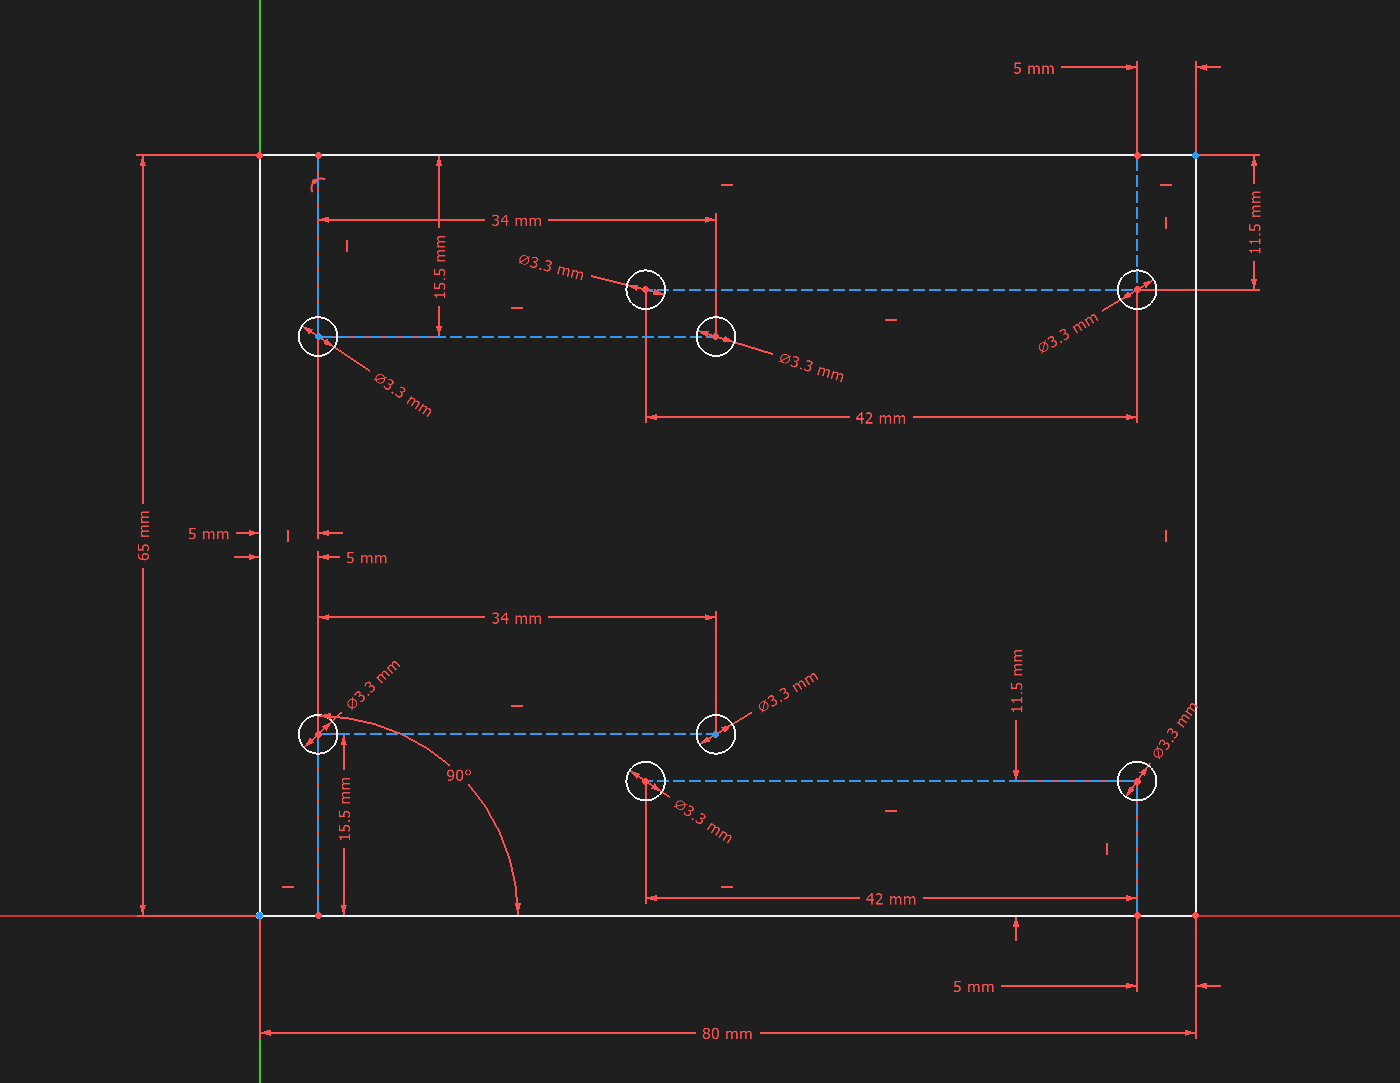
\includegraphics[width=\textwidth]{figures/lidar_mount_sketch.png}
    \caption{Sketch with dimensions in mm.}
  \end{subfigure}\hfill
  \begin{subfigure}[b]{0.40\textwidth}
    \centering
    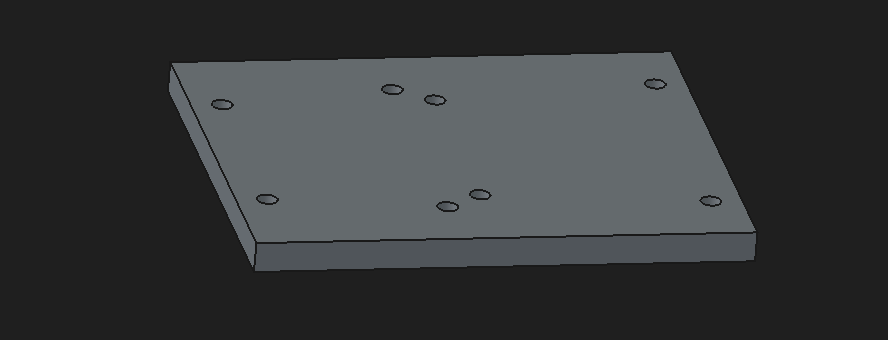
\includegraphics[width=\textwidth]{figures/lidar_mount_3d.png}
    \caption{3D model.}
  \end{subfigure}
  \caption{Adapter plate for the lidar (FreeCAD).}
  \label{fig:mount}
\end{figure}

\paragraph{Position of the lidar.} The position of the lidar relative to \texttt{base\_link} (centre between the wheels on floor level) was measured with a ruler. The centre of the lidar is about \SI{0.01}{\metre} in front of the centre of the robot and in the middle between left and right. The scan plane is about \SI{0.19}{\metre} above the floor. The orientation was checked with the hand test: a hand in front of the robot appeared on the negative $x$-axis of the \texttt{laser} frame, so the lidar is mounted turned by \SI{180}{\degree}. The transform \texttt{base\_link}~$\rightarrow$~\texttt{laser} was therefore set to $(x, y, z) = (0.01, 0, 0.19)\,\si{\metre}$ and yaw $= \pi$.

\section{Mapping and navigation}
\label{sec:slam_method}

\paragraph{Robot description and launch file.} The fixed transforms of the robot were described in a URDF file with the frames \texttt{base\_link}, \texttt{laser} and \texttt{imu\_link} (Appendix~\ref{app:code}). To start the robot with one command, a launch file \texttt{robot.launch.py} was added to the package \texttt{rasprover\_bridge}. It starts the \texttt{robot\_state\_publisher}, the bridge node with the calibrated distance scale, the lidar driver and, if wanted, the \texttt{foxglove\_bridge}. SLAM Toolbox and Nav2 were installed as ROS2 packages. At first, they were started by hand in separate terminals of the same container. Later, a second launch file \texttt{bringup.launch.py} was written, which starts everything with one command: it starts \texttt{robot.launch.py}, then SLAM Toolbox after \SI{5}{\second} and Nav2 after \SI{15}{\second}. The delays make sure that the gyroscope calibration is finished before SLAM Toolbox starts and that SLAM Toolbox already provides the transform \texttt{map}~$\rightarrow$~\texttt{odom} when Nav2 starts. With the argument \texttt{nav:=false}, only the robot and SLAM Toolbox are started, e.g.\ for mapping only.

\paragraph{Nodes.} Fig.~\ref{fig:nodes} shows all nodes and how they are connected. Table~\ref{tab:nodes} explains what each node does.

\begin{figure}[H]
  \centering
  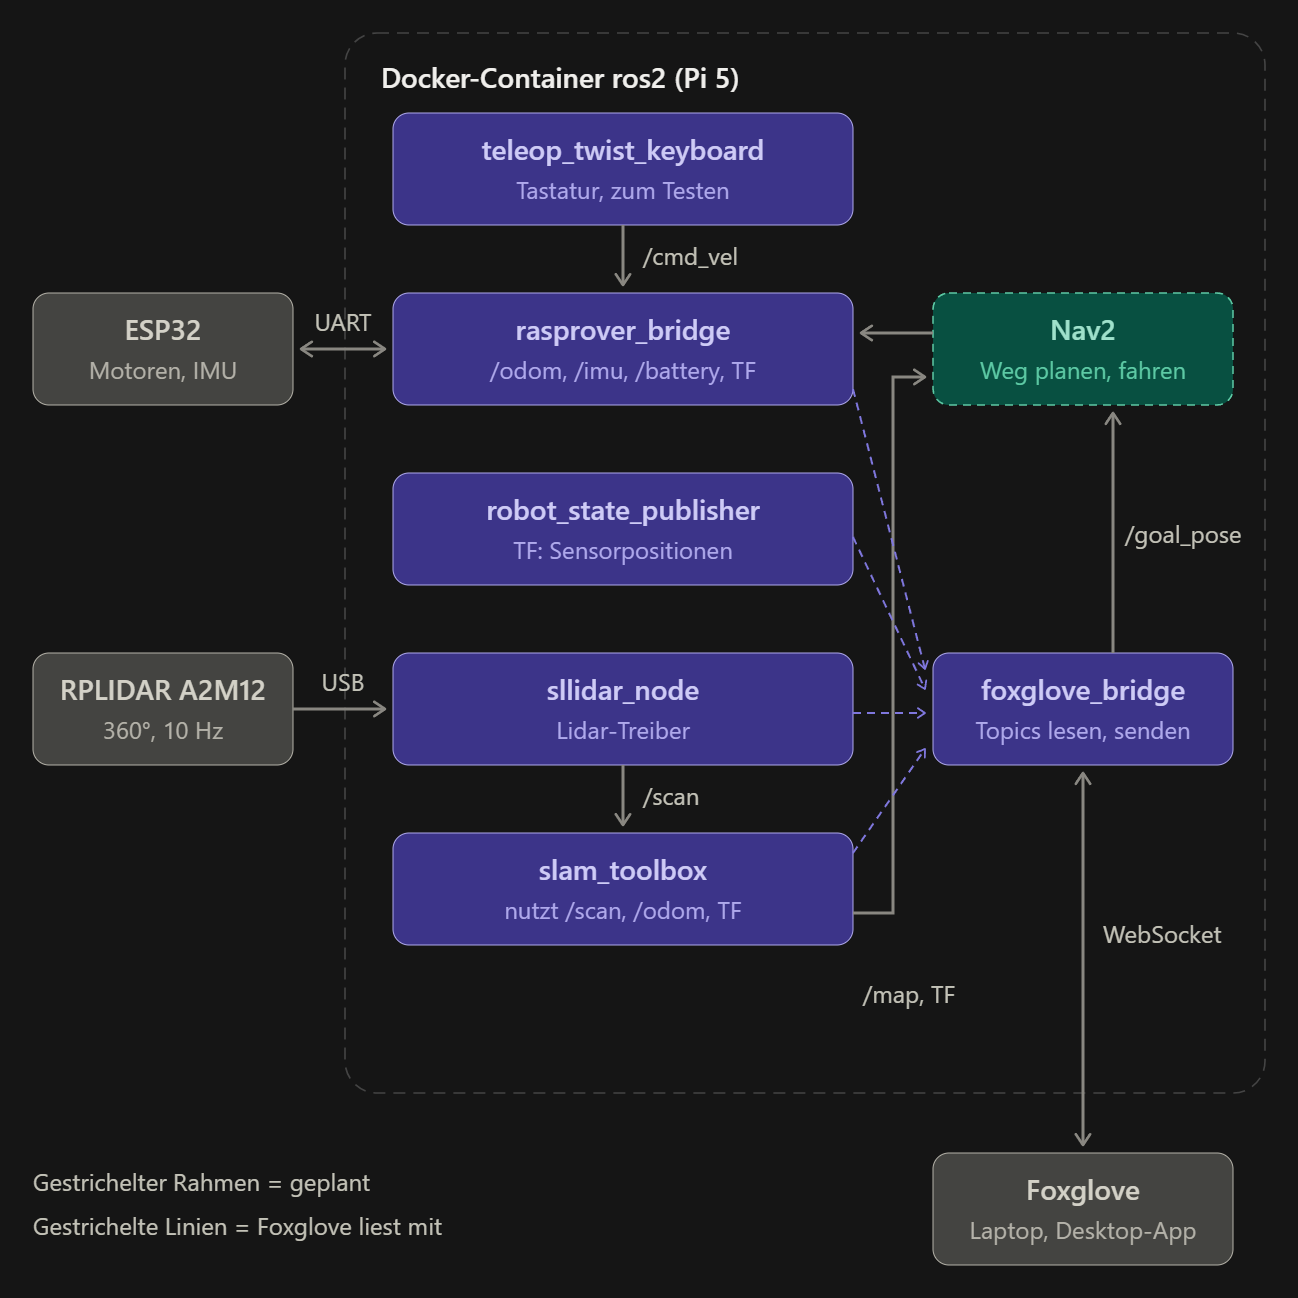
\includegraphics[width=0.85\textwidth]{figures/node_overview.png}
  \caption{Nodes and topics on the robot. \todo{Placeholder, figure will be redrawn.}}
  \label{fig:nodes}
\end{figure}

\begin{table}[H]
  \centering
  \small
  \caption{Nodes used in this work and their function.}
  \label{tab:nodes}
  \begin{tabularx}{\textwidth}{@{}>{\raggedright\arraybackslash}p{3.9cm} X >{\raggedright\arraybackslash}p{3.4cm}@{}}
    \toprule
    \textbf{Node} & \textbf{Function} & \textbf{Topics (in / out)} \\
    \midrule
    \texttt{teleop\_twist\_keyboard} & Drives the robot with the keyboard. Used for tests and for driving while creating the map. & out: \texttt{/cmd\_vel} \\
    \texttt{rasprover\_bridge} & Own node (Section~\ref{sec:bridge}). Sends the drive commands to the ESP32 and publishes the odometry, the IMU values and the battery voltage. & in: \texttt{/cmd\_vel} \newline out: \texttt{/odom}, \texttt{/imu/data\_raw}, \texttt{/battery\_state}, TF \texttt{odom}$\rightarrow$\texttt{base\_link} \\
    \texttt{robot\_state\_publisher} & Reads the URDF file and publishes the fixed positions of the sensors on the robot. & out: TF \texttt{base\_link}$\rightarrow$\texttt{laser}, \texttt{imu\_link} \\
    \texttt{sllidar\_node} & Driver of the lidar. Reads the measurements over USB and publishes them as laser scan. & out: \texttt{/scan} \\
    \texttt{slam\_toolbox} & Creates the map from the laser scans and the odometry and corrects the position of the robot in the map. & in: \texttt{/scan}, TF \newline out: \texttt{/map}, TF \texttt{map}$\rightarrow$\texttt{odom} \\
    Nav2 (several nodes) & Plans a path to the goal, follows it and avoids obstacles (Section~\ref{sec:theory_slam}). & in: \texttt{/goal\_pose}, \texttt{/map}, \texttt{/scan}, \texttt{/odom}, TF \newline out: \texttt{/cmd\_vel} \\
    \texttt{foxglove\_bridge} & Makes the topics available to the Foxglove application on the laptop (WebSocket, port 8765). Foxglove shows the scan, the map and the frames and can send goals. & in/out: all topics, e.g.\ out: \texttt{/goal\_pose} \\
    \bottomrule
  \end{tabularx}
\end{table}

\paragraph{Mapping.} The map was created with SLAM Toolbox in asynchronous online mode. In the configuration, the robot frame was changed from \texttt{base\_footprint} to \texttt{base\_link}, the maximum laser range was set to \SI{12}{\metre} as in the data sheet of the lidar~\citep{slamtec_a2m12}, and the map resolution was set to \SI{0.05}{\metre}. The robot was driven manually with \texttt{teleop\_twist\_keyboard} while the map was checked live in Foxglove. Afterwards, the map was saved with \texttt{map\_saver\_cli} from the package \texttt{nav2\_map\_server}.

\paragraph{Navigation.} Following a suggestion of the supervisor, the robot should be able to navigate and avoid obstacles with only a partial map, because mapping the whole Schlosshof in advance would take a long time. Therefore, Nav2 was started with \texttt{navigation\_launch.py} while SLAM Toolbox was running. In this setup, SLAM Toolbox provides both the map and the position of the robot, as described in the Nav2 documentation~\citep{nav2_slam}. Because the map grows while the robot drives, the planner was allowed to plan through unknown areas (\texttt{allow\_unknown: true}). In the Nav2 configuration, the robot frame was changed to \texttt{base\_link}, and the MPPI controller was used. To save computing power on the Raspberry Pi, the number of sampled trajectories of the MPPI controller (\texttt{batch\_size}) was reduced to 1000 and its visualisation was switched off. Goals were set in Foxglove with the \emph{2D pose} tool of the 3D panel, which publishes a pose on \texttt{/goal\_pose}.

For the cost maps, the robot is described as a circle around \texttt{base\_link}. The robot is about \SI{20}{\centi\metre} long and \SI{18}{\centi\metre} wide (measured with a small buffer), which gives a radius of $\sqrt{0.10^2 + 0.09^2} \approx \SI{0.14}{\metre}$. The safety zone around obstacles (\texttt{inflation\_radius}) was reduced from \SI{0.70}{\metre} to \SI{0.30}{\metre}, because with the larger values the robot could hardly move in a small room (Section~\ref{sec:nav_results}). For the first tests, low velocity and acceleration limits were used, which were increased after the first tests (Tab.~\ref{tab:nav2}).

Because the MPPI controller turned the robot with several small forward and backward movements instead of turning on the spot, the Rotation Shim Controller of Nav2 was added in front of it. If the path points more than \SI{45}{\degree} away from the heading of the robot, it first turns the robot on the spot with a commanded angular velocity of \SI{1.6}{\radian\per\second} and then hands over to the MPPI controller. Its angular acceleration limit was first set to \SI{2.5}{\radian\per\second\squared} and then increased to \SI{10}{\radian\per\second\squared} (Section~\ref{sec:nav_results}). The shim was also set to turn the robot into the final orientation at the goal (\texttt{rotate\_to\_goal\_heading}), because the MPPI controller turned the robot back and forth at the goal.

The log of Nav2 showed that the controller could not keep its rate of \SI{20}{\hertz} on the Raspberry Pi. The controller rate was therefore reduced to \SI{10}{\hertz}. So that the MPPI controller still plans \SI{2.8}{\second} ahead, its time step (\texttt{model\_dt}) was increased from \SI{0.05}{\second} to \SI{0.1}{\second} and the number of time steps was reduced from 56 to 28. In addition, Nav2 aborted goals during slow manoeuvres around obstacles because the progress checker did not detect enough progress. Its limits were therefore relaxed from \SI{0.5}{\metre} in \SI{10}{\second} to \SI{0.25}{\metre} in \SI{20}{\second}.

\begin{table}[H]
  \centering
  \small
  \caption{Nav2 parameters in the first tests and after the adjustments.}
  \label{tab:nav2}
  \begin{tabular}{@{}lll@{}}
    \toprule
    \textbf{Parameter} & \textbf{First tests} & \textbf{Adjusted} \\
    \midrule
    Max.\ linear velocity & \SI{0.25}{\metre\per\second} & \SI{0.4}{\metre\per\second} \\
    Min.\ linear velocity (reverse) & \SI{-0.15}{\metre\per\second} & \SI{-0.15}{\metre\per\second} \\
    Max.\ angular velocity & \SI{1.2}{\radian\per\second} & \SI{1.6}{\radian\per\second} \\
    Max.\ linear acceleration / deceleration & $\pm$\SI{1.0}{\metre\per\second\squared} & $\pm$\SI{1.5}{\metre\per\second\squared} \\
    Max.\ angular acceleration / deceleration & $\pm$\SI{2.0}{\radian\per\second\squared} & $\pm$\SI{2.5}{\radian\per\second\squared} \\
    Robot radius & \SI{0.22}{\metre} & \SI{0.14}{\metre} \\
    Inflation radius & \SI{0.70}{\metre} & \SI{0.30}{\metre} \\
    Rotation Shim Controller & -- & \SI{1.6}{\radian\per\second}, \SI{10}{\radian\per\second\squared} \\
    Rotation to goal heading by shim & -- & yes \\
    Controller rate & \SI{20}{\hertz} & \SI{10}{\hertz} \\
    MPPI time step / number of steps & \SI{0.05}{\second} / 56 & \SI{0.1}{\second} / 28 \\
    Progress checker & \SI{0.5}{\metre} in \SI{10}{\second} & \SI{0.25}{\metre} in \SI{20}{\second} \\
    \bottomrule
  \end{tabular}
\end{table}

The velocity and acceleration limits were set both in the MPPI controller and in the velocity smoother. The commands for starting the system are listed in Appendix~\ref{app:commands}.

\paragraph{Exploration.} For autonomous mapping, the package \texttt{explore\_lite} (ROS2 version \texttt{m-explore-ros2}) was used~\citep{m_explore}. It is not available as a binary package for ROS2 Jazzy, so it was built from source in the container, together with its message package \texttt{explore\_lite\_msgs}. It was started with its default parameters in a separate terminal after \texttt{bringup.launch.py}, as soon as Nav2 was ready. The frontiers were shown in Foxglove on the topic \texttt{/explore/frontiers}. Because the lidar only measures in one plane, open doors were closed off with a light-coloured obstacle higher than \SI{20}{\centi\metre}, so that the robot does not leave the test area.

\section{Evaluation}
\label{sec:evaluation_method}

The final tests are carried out in the Schlosshof, as planned in the project outline. Before that, the procedure was tested indoors. \todo{Adapt to the final test plan in the Schlosshof.}

\paragraph{Exploration and map.} The robot explores the test area with \texttt{explore\_lite} until no reachable frontiers are left. The duration and the number of goals are taken from the log. To evaluate the map accuracy, distances between clearly visible points (e.g.\ walls, pillars) are measured in the saved map and compared with measurements with a measuring tape. \todo{Points and distances.}

\paragraph{Reaching goals.} In the finished map, goals are set repeatedly from the same start position. For each run, it is recorded whether the goal is reached, the time between \texttt{Begin navigating} and \texttt{Goal succeeded} in the log, the number of \texttt{Failed to make progress} messages and the distance between the robot and the goal position, measured with a measuring tape. \todo{Number of goals and repetitions.}

\paragraph{Obstacle avoidance.} To test whether the robot avoids obstacles without a complete map, the robot is first driven to a place from where it cannot see a certain part of the area. An obstacle is placed there, and a goal behind the obstacle is set. The obstacle has to be higher than \SI{20}{\centi\metre}, because the lidar only measures in one plane at \SI{0.19}{\metre} above the floor. It is observed whether the robot detects the obstacle, plans a new path around it and reaches the goal. For this, the local cost map, the planned path (\texttt{/plan}) and the scan are shown in Foxglove. \todo{Obstacles (light and dark), number of repetitions.}

\chapter{Results}
\label{ch:results}

\section{Commissioning}
\label{sec:commissioning}

At the beginning, the Raspberry Pi only booted with an external power supply, and drive commands from the web application were not executed, although the web application showed the battery voltage. A test over the Wi-Fi interface of the ESP32 showed that the ESP32 and the motors worked. The problem was that the Raspberry Pi had been mounted the wrong way round, so its 40-pin header was not plugged into the driver board and neither the \SI{5}{\volt} supply nor the UART connection worked. After mounting it correctly, the Pi booted from the battery and executed the drive commands. After the re-assembly, the camera was not detected anymore; reconnecting its cables fixed this.

ROS2 Jazzy was installed in the Docker container as described in Section~\ref{sec:software}. The installation was tested with the talker/listener example and with a serial test from the container, in which the wheels turned and a feedback message was received.

\section{Meaning of the ESP32 feedback}
\label{sec:feedback_results}

Table~\ref{tab:feedback} shows the meaning and conversion of the feedback values determined in the calibration tests. The measured values are in Appendix~\ref{app:rawdata}.

\begin{table}[H]
  \centering
  \small
  \caption{Values of the ESP32 feedback message and their conversion to SI units ($b$: gyroscope offset, $g$: gravitational acceleration).}
  \label{tab:feedback}
  \begin{tabularx}{\textwidth}{@{}l X >{\raggedright\arraybackslash}p{3.8cm}@{}}
    \toprule
    \textbf{Value} & \textbf{Meaning} & \textbf{Conversion} \\
    \midrule
    \texttt{L}, \texttt{R}        & Speed of the left / right side & direct, \si{\metre\per\second} \\
    \texttt{odl}, \texttt{odr}    & Distance of the left / right side; integer, adds up, signed, reset at ESP32 restart & $\times\,0.0097$ $\rightarrow$ \si{\metre} \\
    \texttt{ax}, \texttt{ay}, \texttt{az} & Acceleration, raw values & $/\,8192 \cdot g$ $\rightarrow$ \si{\metre\per\second\squared} \\
    \texttt{gx}, \texttt{gy}, \texttt{gz} & Angular rate, raw values & $(\text{raw} - b)/16.4$ $\rightarrow$ \si{\degree\per\second} \\
    \texttt{mx}, \texttt{my}, \texttt{mz} & Magnetic field, raw values & not used \\
    \texttt{v}                    & Battery voltage & $/\,100$ $\rightarrow$ \si{\volt} \\
    \bottomrule
  \end{tabularx}
\end{table}

\section{Calibration}
\label{sec:calibration_results}

\paragraph{Wheel speed and distance.} With a commanded speed of \SI{0.3}{\metre\per\second}, \texttt{L}/\texttt{R} showed \SI{0.299}{\metre\per\second}. Driving forward for about \SI{95}{\centi\metre} increased \texttt{odl}/\texttt{odr} by 97 and 98, about 15 per \SI{0.5}{\second}. Driving backward over a similar distance changed them by $-99$ and $-98$. Between two tests, the counters jumped from 384 to 175 without any movement. In a first attempt without clearing the input buffer, a change of only 1 was measured for the same drive.

\paragraph{Accelerometer.} When the robot was standing, the vertical axis showed $a_z = 8156$. Upside down, it showed $a_z = -8462$.

\paragraph{Gyroscope.} The offset of the vertical axis was $b_z = 6.6$ (30 values), which is \SI{0.40}{\degree\per\second}. In the turn test, the integrated values (without offset) were \num{1930.3} raw units$\cdot$\si{\second} for an estimated rotation of \SI{120}{\degree}. This gives a scale factor of $1930.3/120 \approx 16.1$ raw units per \si{\degree\per\second}. The mean value during the turn was 730 raw units, i.e.\ \SI{44.5}{\degree\per\second} or \SI{0.78}{\radian\per\second}. This is only \SI{52}{\percent} of the commanded \SI{1.5}{\radian\per\second}.

Table~\ref{tab:calibration} shows the values that were used in the bridge node.

\begin{table}[H]
  \centering
  \small
  \caption{Calibration values used in the bridge node.}
  \label{tab:calibration}
  \begin{tabular}{@{}l l l@{}}
    \toprule
    \textbf{Parameter} & \textbf{Value} & \textbf{Based on} \\
    \midrule
    Distance scale $s$      & \SI{0.0097}{\metre} per unit     & distance tests, straight drive \\
    Accelerometer scale     & 8192 per $g$                     & value while standing \\
    Gyroscope scale         & 16.4 per \si{\degree\per\second} & turn test (16.1) \\
    Gyroscope offset $b_z$  & measured at every start          & mean over \SI{2}{\second} while standing \\
    \bottomrule
  \end{tabular}
\end{table}

\section{Test of the bridge node}
\label{sec:validation_results}

\paragraph{Rate.} \texttt{/odom} was published with \SI{19.8}{\hertz} on average, with time steps between \SI{50}{\milli\second} and \SI{57}{\milli\second} (standard deviation about \SI{1}{\milli\second}). At the start, the node measured a gyroscope offset of $b_z = 6.7$ from 43 values. The robot followed the keyboard commands without interruptions.

\paragraph{Straight drive and turn.} Table~\ref{tab:validation} compares the odometry with the measured or estimated movement. For the straight drive, the first scale factor of \SI{0.01}{\metre} per unit was still used.

\begin{table}[H]
  \centering
  \small
  \caption{Odometry compared with the measured movement.}
  \label{tab:validation}
  \begin{tabular}{@{}l l r l@{}}
    \toprule
    \textbf{Test} & \textbf{Value} & \textbf{Odometry} & \textbf{Measured / estimated} \\
    \midrule
    Straight drive & Distance $x$       & \SI{1.084}{\metre}  & about \SI{1.05}{\metre} \\
                   & Lateral offset $y$ & \SI{-0.028}{\metre} & slight drift to the right \\
                   & Heading $\psi$     & \SI{-4.4}{\degree}  & slight turn to the right \\
    \midrule
    Turn           & Heading, start     & \SI{-10.4}{\degree} ($q_z = -0.0905$) & -- \\
                   & Heading, end       & \SI{86.7}{\degree} ($q_z = 0.6865$)  & -- \\
                   & Rotation           & \SI{97.1}{\degree}  & a bit more than \SI{90}{\degree} \\
    \bottomrule
  \end{tabular}
\end{table}

The odometry overestimated the distance by about \SI{3}{\percent}, so the scale factor was changed to \SI{0.0097}{\metre} per unit. While standing still, the heading changed by about \SI{0.1}{\degree} in \SI{4}{\second} after the straight drive and by about \SI{0.3}{\degree} in \SI{9}{\second} before the turn. This corresponds to a remaining drift of about \SI{0.03}{\degree\per\second}.

\section{Lidar integration}
\label{sec:lidar_results}

At the first start, the driver connected to the lidar and read its serial number, firmware version (1.32) and health status (OK), but the scan could not be started (error code \texttt{80008002}, timeout), and the lidar motor did not turn. At the same time, the kernel log showed that the USB camera was disconnected and connected again, which points to a voltage drop on the USB ports. The USB current limit of the Raspberry Pi was active (\texttt{usb\_max\_current\_enable=0}). After switching off the limit and restarting, the motor turned, the scan ran without errors, and no undervoltage was reported (\texttt{throttled=0x0}). In addition, the launch file of the driver for the A2M12 had a space in its file name and had to be renamed before it could be used.

The scan was published with \SI{10.1}{\hertz} on average (time steps \SIrange{0.092}{0.105}{\second}, standard deviation about \SI{2}{\milli\second}). A hand held close to the lidar appeared as a group of points at the expected distance of about \SIrange{0.15}{0.35}{\metre}. When the robot was standing on a table, many directions gave no measurement (\texttt{inf}), because the scan plane was just above the table. In the visualisation, an object in front of the robot appeared on the negative $x$-axis, which showed that the lidar is turned by \SI{180}{\degree} (raw data in Appendix~\ref{app:rawdata}). After mounting the lidar with the adapter plate and setting yaw $=\pi$ in the URDF, objects in front of the robot were shown in front of the robot model.

\section{Mapping and navigation}
\label{sec:nav_results}

\todo{Write at the end. Notes so far:
\begin{itemize}
  \item First indoor map created and saved (\texttt{raum1}); screenshot still missing.
  \item Slowly growing offset between \texttt{odom} and \texttt{base\_link} visible in Foxglove (gyro drift), corrected by SLAM Toolbox via \texttt{map}~$\rightarrow$~\texttt{odom}.
  \item Start problem: Nav2 reported missing transform \texttt{base\_link}~$\rightarrow$~\texttt{map}, SLAM Toolbox dropped scans (``Message Filter dropping message''). Cause: \texttt{robot\_state\_publisher} not running. Fixed by restart and fixed start order.
  \item Two goals set in Foxglove were reached.
  \item Problems: ``Failed to make progress'' with recovery behaviours, jerky driving at low velocities, occasional ``control loop missed its desired rate''.
  \item \texttt{bringup.launch.py}: all nodes start. \texttt{ros2 node list} first showed only part of the nodes; after \texttt{ros2 daemon stop} all nodes were listed.
  \item Small room with robot radius \SI{0.22}{\metre} and inflation radius \SI{0.70}{\metre}: robot hardly moved, area around it was treated as blocked.
  \item Higher velocity limits: driving straight much smoother. Turning: stuttering forward and backward movements instead of turning on the spot.
  \item Constant command \SI{1.6}{\radian\per\second} with \texttt{ros2 topic pub} (without Nav2): robot turns smoothly on the spot $\rightarrow$ hardware OK.
  \item Rotation Shim Controller: robot turns on the spot, but with interruptions at \SI{2.5}{\radian\per\second\squared}; much better at \SI{10}{\radian\per\second\squared}.
  \item Obstacle test (living room): obstacle detected, robot drives around it and reaches the goal, but sometimes stands still for several seconds, and the detour takes very long. Cause still open (log analysis and CPU load planned).
  \item Still to do: analyse standstill in obstacle test, repeated runs (success rate, position error), map accuracy, exploration (\texttt{explore\_lite}), Schlosshof.
\end{itemize}}

\chapter{Discussion}
\label{ch:discussion}

\section{Odometry and calibration}

\todo{Write at the end. Notes:
\begin{itemize}
  \item Accelerometer: 8156 at standstill fits 8192 per $g$.
  \item Gyroscope scale: turn test 16.1, 16.4 used because the angle was only estimated; test turn 97° for slightly more than 90°.
  \item Distance error 3\,\% in two tests, corrected; counter resolution 1\,cm.
  \item Slip when turning: only 52\,\% of commanded rate $\rightarrow$ heading from gyroscope instead of wheels.
  \item Remaining drift approx.\ 2°/min (24°/min without offset correction), corrected by SLAM.
  \item Limits: short tests, one smooth floor, estimates by eye; gravel/grass in the Schlosshof will differ.
\end{itemize}}

\section{Platform and software}

\todo{Write at the end. Notes:
\begin{itemize}
  \item Commercial platform solved open points of the previous work (encoders, IMU, motor controller), but firmware is poorly documented.
  \item Docker: manufacturer image unchanged, but privileged container; Dockerfile still missing.
  \item Power supply: USB current limit, highest load when motors, lidar and Pi run together.
  \item Simple Python bridge node instead of \texttt{ros2\_control}; two independent stop functions.
\end{itemize}}

\section{Mapping and navigation}

\todo{Write at the end (map quality, localisation, obstacle avoidance, reaching goals, computing load on the Raspberry Pi). Notes:
\begin{itemize}
  \item Default robot radius and inflation radius too large for small rooms; values have to fit the real robot size.
  \item MPPI with skid steering: turning in several small moves; Rotation Shim Controller makes turning on the spot possible.
  \item Possible reason for the stuttering at low angular acceleration: the shim increases the command step by step starting from the measured angular velocity, the robot turns slower than commanded (slip, 52\,\%), so the commands stay too low to start the rotation. Still to be checked.
  \item Supervisor: robot should work with partial maps and avoid obstacles without knowing the whole area (Schlosshof is large). Nav2 already works with the growing SLAM map and the live scan in the local cost map.
  \item Standstill during obstacle avoidance: commands near obstacles very small, Pi could not keep \SI{20}{\hertz}; after reducing to \SI{10}{\hertz} and relaxing the progress checker clearly better (goals in under \SI{25}{\second} instead of over \SI{1}{\minute}).
  \item Dark, matte obstacle: robot turned on the spot repeatedly; possibly the lidar does not detect the box reliably (low reflection). To be checked in the scan.
  \item Exploration works in a closed room: map created autonomously in about \SI{2}{\minute}.
  \item 2D lidar does not see low obstacles or edges (door threshold, kerbs): robot fell over the door threshold. Open areas have to be closed off physically; possible improvements: virtual walls (keepout zones) or an additional sensor pointing at the floor.
  \item Schlosshof: larger area, open passages, uneven ground (link to challenges in Section~\ref{sec:challenges}).
\end{itemize}}

\section{Achievement of objectives}

\todo{Write at the end (status of objectives 1 and 2 and of the evaluation, deviations from the plan).}

\section{Reflection on the work process}

\todo{Personal reflection.}

\section{Outlook}

\todo{Write at the end.}


% References: numbered chapter (guideline), numeric in order of citation
\bibliographystyle{unsrtnat}
\bibliography{references}

% ---------------- Lists (not numbered) ----------------------
\cleardoublepage
\phantomsection
\addcontentsline{toc}{chapter}{List of Figures}
\listoffigures
\phantomsection
\addcontentsline{toc}{chapter}{List of Tables}
\listoftables

% ---------------- Appendix (not numbered) -------------------
\appendix
% Appendix directory at the beginning of the appendix (guideline 3.1.12).
% Page and chapter numbering are not continued in the appendix.
\cleardoublepage
\pagenumbering{Roman}
\chapter*{Appendix}
\phantomsection
\addcontentsline{toc}{chapter}{Appendix}
\thispagestyle{fancy}

\begin{tabularx}{\textwidth}{@{}l X r@{}}
  \toprule
  \textbf{Appendix} & \textbf{Content} & \textbf{Page} \\
  \midrule
  A & Directory of the generative AI systems used & \pageref{app:ai} \\
  B & Command reference (ESP32 and ROS2) & \pageref{app:commands} \\
  C & Raw data of the calibration and validation tests & \pageref{app:rawdata} \\
  D & Source code (bridge node, URDF, launch file) & \pageref{app:code} \\
  E & Declaration of originality & \pageref{app:declaration} \\
  \bottomrule
\end{tabularx}

% Appendix chapters are not listed individually in the table of contents
\addtocontents{toc}{\protect\setcounter{tocdepth}{-1}}

\chapter{Directory of the Generative AI Systems Used}
\label{app:ai}

Declaration according to the ZHAW information sheet on the use of generative AI in assignments (version 2.0.0). The author remains responsible for the relevance, correctness and accuracy of all content; all AI output was checked, and all measurements and tests on the robot were carried out by the author.

\todo{Information duty: ask the supervisor which use of generative AI is expected or allowed and in which form it has to be declared; adapt this table accordingly.}

\begin{table}[H]
  \centering
  \small
  \caption{Generative AI systems used, purpose and area of application.}
  \label{tab:ai}
  \begin{tabularx}{\textwidth}{@{}>{\raggedright\arraybackslash}p{4.2cm} X >{\raggedright\arraybackslash}p{3.6cm}@{}}
    \toprule
    \textbf{AI system} & \textbf{Purpose} & \textbf{Area of application} \\
    \midrule
    Anthropic. (2026). \emph{Claude} [Large language model]. https://claude.ai
      & Support with troubleshooting during commissioning
      & Sections~\ref{sec:commissioning}, \ref{sec:lidar_results} and~\ref{sec:nav_results} \\
    & Generation of source code (bridge node, test scripts, URDF, launch file) and of the SLAM and Nav2 configuration
      & Sections~\ref{sec:bridge} and~\ref{sec:slam_method}, Appendix~\ref{app:code} \\
    & Structuring, formulation and translation of the text
      & Entire work \\
    \bottomrule
  \end{tabularx}
\end{table}

\chapter{Command Reference}
\label{app:commands}

Selection of JSON commands of the ESP32 firmware. All commands are documented by Waveshare~\citep{waveshare_json}.

\begin{table}[H]
  \centering
  \small
  \caption{Selected ESP32 commands.}
  \label{tab:commandref}
  \begin{tabularx}{\textwidth}{@{}l X@{}}
    \toprule
    \textbf{Command} & \textbf{Function} \\
    \midrule
    \multicolumn{2}{@{}l}{\textit{Motion}} \\
    \texttt{\{"T":1,"L":0.2,"R":0.2\}}         & Target speed left / right in \si{\metre\per\second} (closed loop) \\
    \texttt{\{"T":11,"L":164,"R":164\}}        & PWM value left / right, $-255$ to $255$ (open loop) \\
    \texttt{\{"T":13,"X":0.1,"Z":0.3\}}        & Linear (\si{\metre\per\second}) and angular (\si{\radian\per\second}) velocity \\
    \texttt{\{"T":2,"P":20,"I":2000,"D":0,"L":255\}} & PID parameters of the motor controller (default values) \\
    \texttt{\{"T":138,"L":1,"R":1\}}           & Speed ratio left / right for straight driving \\
    \texttt{\{"T":136,"cmd":3000\}}            & Heartbeat interval in \si{\milli\second} \\
    \midrule
    \multicolumn{2}{@{}l}{\textit{Feedback and sensors}} \\
    \texttt{\{"T":130\}}                       & Request a single feedback message \\
    \texttt{\{"T":131,"cmd":1\}}               & Continuous feedback on (1) / off (0) \\
    \texttt{\{"T":142,"cmd":50\}}              & Feedback interval in \si{\milli\second} \\
    \texttt{\{"T":126\}}                       & Request IMU data \\
    \texttt{\{"T":143,"cmd":1\}}               & Echo received commands (debugging) \\
    \midrule
    \multicolumn{2}{@{}l}{\textit{Configuration and output}} \\
    \texttt{\{"T":900,"main":1,"module":0\}}   & Chassis type (1 = RaspRover) and module (0 = none) \\
    \texttt{\{"T":3,"lineNum":0,"Text":"..."\}} & Text on the OLED display (lines 0--3) \\
    \texttt{\{"T":132,"IO4":255,"IO5":255\}}   & 12\,V switched outputs / LEDs, 0--255 \\
    \texttt{\{"T":600\}}                       & Restart the ESP32 \\
    \bottomrule
  \end{tabularx}
\end{table}

\section*{ROS2 commands}

Commands used to start the system in the container (\texttt{docker exec -it ros2 bash}). Normally, everything is started with one command:

\begin{lstlisting}[language=bash, numbers=none, caption={Start with one command.}, label={lst:bringup}]
# Robot, SLAM Toolbox (after 5 s) and Nav2 (after 15 s)
ros2 launch rasprover_bridge bringup.launch.py
# Only robot and SLAM Toolbox (mapping)
ros2 launch rasprover_bridge bringup.launch.py nav:=false
# Save the log at the same time
ros2 launch rasprover_bridge bringup.launch.py 2>&1 | tee /ros2_ws/nav_log.txt
\end{lstlisting}

For troubleshooting, the parts can also be started one by one, each in its own terminal:

\begin{lstlisting}[language=bash, numbers=none, caption={Start step by step.}, label={lst:start}]
# 1. Robot: robot_state_publisher, bridge node, lidar, foxglove_bridge
ros2 launch rasprover_bridge robot.launch.py
# 2. SLAM Toolbox
ros2 launch slam_toolbox online_async_launch.py \
  slam_params_file:=/ros2_ws/config/slam.yaml
# 3. Check the transform tree
ros2 run tf2_ros tf2_echo map base_link
# 4. Nav2
ros2 launch nav2_bringup navigation_launch.py \
  params_file:=/ros2_ws/config/nav2.yaml
\end{lstlisting}

\begin{lstlisting}[language=bash, numbers=none, caption={Other commands.}, label={lst:other}]
# Manual driving
ros2 run teleop_twist_keyboard teleop_twist_keyboard
# Constant rotation for testing (stop with Ctrl+C)
ros2 topic pub -r 10 /cmd_vel geometry_msgs/msg/Twist "{angular: {z: 1.6}}"
# Save the map
ros2 run nav2_map_server map_saver_cli -f /ros2_ws/maps/raum1
# List running nodes (restart the daemon if the list is incomplete)
ros2 daemon stop
ros2 node list
\end{lstlisting}

\chapter{Raw Data of the Calibration and Validation Tests}
\label{app:rawdata}

\section*{C.1 Feedback message at standstill}

\begin{lstlisting}[language=json, numbers=none, caption={Feedback message of the ESP32 at standstill.}, label={lst:feedback}]
{"T":1001,"L":0,"R":0,"ax":12,"ay":-118,"az":8156,"gx":-46,"gy":20,"gz":8,
 "mx":-428,"my":8,"mz":899,"odl":44,"odr":55,"v":1167}
\end{lstlisting}

\section*{C.2 Distance tests}

Commanded speed \SI{0.3}{\metre\per\second} on both sides; values printed every fifth command (approx.\ \SI{0.5}{\second}).

\begin{lstlisting}[numbers=none, caption={Forward drive, measured distance approx.\ 95\,cm.}, label={lst:forward}]
Start: 276 286
0 L: 0 R: 0 odl: 276 odr: 286
5 L: 0.2991993 R: 0.2991993 odl: 288 odr: 298
10 L: 0.2991993 R: 0.2991993 odl: 303 odr: 314
15 L: 0.2991993 R: 0.299049775 odl: 319 odr: 329
20 L: 0.2991993 R: 0.2991993 odl: 334 odr: 345
25 L: 0.2991993 R: 0.35903916 odl: 349 odr: 360
30 L: 0.2991993 R: 0.299949173 odl: 364 odr: 375
End: 373 384
Difference odl: 97 odr: 98
\end{lstlisting}

\begin{lstlisting}[numbers=none, caption={Backward drive over a similar distance.}, label={lst:backward}]
Start: 175 184
0 L: -0.11967972 R: -0.11961991 odl: 174 odr: 183
5 L: -0.2991993 R: -0.2991993 odl: 160 odr: 170
10 L: -0.2991993 R: -0.2991993 odl: 145 odr: 154
15 L: -0.2991993 R: -0.284061797 odl: 129 odr: 139
20 L: -0.35903916 R: -0.2991993 odl: 114 odr: 124
25 L: -0.2991993 R: -0.23935944 odl: 99 odr: 109
30 L: -0.2991993 R: -0.299348975 odl: 84 odr: 94
End: 76 86
Difference odl: -99 odr: -98
\end{lstlisting}

\section*{C.3 Gyroscope tests}

\begin{lstlisting}[numbers=none, caption={Gyroscope offset and turn test (commanded 1.5\,rad/s for 3\,s, estimated rotation approx.\ 120\textdegree).}, label={lst:gyro}]
Gyro offset gz (standstill): 6.6
Number of samples: 80
Mean gz during the turn (raw): 730.0
Integral of gz over time (raw*s): 1930.3
\end{lstlisting}

\section*{C.4 Validation of the bridge node}

\begin{lstlisting}[numbers=none, caption={Publication rate of /odom (excerpt of ros2 topic hz).}, label={lst:hz}]
average rate: 19.815
        min: 0.050s max: 0.053s std dev: 0.00079s window: 21
average rate: 19.757
        min: 0.050s max: 0.057s std dev: 0.00113s window: 181
\end{lstlisting}

\begin{lstlisting}[numbers=none, caption={Gyroscope offset determined by the bridge node at start-up.}, label={lst:nodeoffset}]
Gyro offset determined (43 samples): gx=-50.9 gy=13.3 gz=6.7
\end{lstlisting}

\begin{lstlisting}[numbers=none, caption={Pose on /odom at the end of the straight drive (scale factor 0.01\,m per unit).}, label={lst:straight}]
position:    x: 1.0840747670157718   y: -0.028124860572776945
orientation: z: -0.0380   (standstill, start) ... -0.0392 (approx. 4 s later)
\end{lstlisting}

\begin{lstlisting}[numbers=none, caption={Orientation q\_z on /odom during the turn test (excerpt).}, label={lst:turn}]
before the turn (approx. 9 s standstill): -0.0905 ... -0.0931
end of the turn (standstill):              0.6865 ...  0.6863
\end{lstlisting}

\section*{C.5 Lidar integration}

\begin{lstlisting}[numbers=none, caption={First start of the lidar driver (USB current limit active).}, label={lst:lidarerror}]
[sllidar_node]: SLLidar S/N: 98CDFA89C7E19EC8BCE499F0131A5670
[sllidar_node]: Firmware Ver: 1.32
[sllidar_node]: Hardware Rev: 6
[sllidar_node]: SLLidar health status : OK.
[sllidar_node]: Can not start scan: 80008002!
\end{lstlisting}

\begin{lstlisting}[numbers=none, caption={Publication rate of /scan after lifting the USB current limit (excerpt).}, label={lst:scanhz}]
average rate: 10.073
        min: 0.098s max: 0.104s std dev: 0.00228s window: 12
average rate: 10.105
        min: 0.092s max: 0.105s std dev: 0.00205s window: 177
\end{lstlisting}

\todo{Store the complete recordings (e.g.\ as rosbag or text files) in the repository and refer to them here.}

\chapter{Source Code}
\label{app:code}

The bridge node is a ROS2 Python package (\texttt{ament\_python}) named \texttt{rasprover\_bridge}. It is built with \texttt{colcon build} inside the ROS2 container and started with \texttt{ros2 run rasprover\_bridge bridge}. The calibrated distance scale is passed as parameter: \texttt{--ros-args -p odom\_scale:=0.0097}.

The container was created with the following command on the Raspberry Pi:

\begin{lstlisting}[language=bash, numbers=none, caption={Creation of the ROS2 container.}, label={lst:docker}]
docker run -it --name ros2 \
  --network host --ipc host \
  --privileged -v /dev:/dev \
  -v ~/ros2_ws:/ros2_ws \
  ros:jazzy-ros-base bash
\end{lstlisting}

\lstinputlisting[language=Python, caption={\texttt{bridge\_node.py}}, label={lst:bridge}]{code/bridge_node.py}

\lstinputlisting[language=XML, caption={Robot description \texttt{rasprover.urdf}}, label={lst:urdf}]{code/rasprover_bridge/rasprover.urdf}

\lstinputlisting[language=Python, caption={Launch file \texttt{robot.launch.py}}, label={lst:launch}]{code/rasprover_bridge/robot.launch.py}

\lstinputlisting[language=Python, caption={Launch file \texttt{bringup.launch.py}}, label={lst:bringuplaunch}]{code/rasprover_bridge/bringup.launch.py}

\chapter{Declaration of Originality}
\label{app:declaration}

\todo{Insert the official, signed declaration of originality of the LSFM department here, e.g.\ as PDF page using the package pdfpages.}


\end{document}
